\documentclass{article}

\usepackage{geometry}
\geometry{left=3cm,right=3cm,top=2cm,bottom=2cm}
\usepackage[utf8]{inputenc}
\usepackage{amsmath, amsfonts, amssymb, amsthm}
\usepackage[framemethod=default]{mdframed}% was framemethod=TikZ
\usepackage{mathrsfs}
\usepackage{comment}
\usepackage{enumerate}
\usepackage{xcolor}
\usepackage{titlesec}
\usepackage{setspace}
\usepackage{hyperref}
\hypersetup{
colorlinks=true,
allcolors=orange
}
\usepackage{cleveref}

\usepackage[most]{tcolorbox}
\usepackage{ragged2e}
\usepackage{todonotes}
\usepackage{cleveref}
\usepackage{mathtools}
\usepackage{svg, float}

\usepackage[sectionbib]{natbib}
\usepackage{chapterbib}


\definecolor{astral}        {RGB}{46,116,181}
\definecolor{cb-blue}       {RGB}{70, 130, 180}
\definecolor{orange}        {RGB}{214,150, 92}


% Name of the author!!!
\newcommand{\aut}{AUTHOR}

%
\titleformat*{\section}{\LARGE \bfseries}
\titleformat*{\subsection}{\Large \bfseries}
\titleformat*{\subsubsection}{\Large \bfseries}
% \titleformat*{\paragraph}{\large \bfseries}
\titleformat*{\subparagraph}{\large \bfseries}


%%%%%%%%%%%%%%%%%%%%%%%%%%%%%%%%%%%%%%%%%%%%%%%%%%%%%%%%%%%%
% General 
\newcommand{\nextline}{\hfill\break}
\newcommand{\nl}{\nextline\rm}
% \newcommand{\placeholder}{{\bf\color{red} NOOOOOOT COMPLEEEEEEET! COOOOOOOM BAAAAAACK!!!}}
\newcommand{\placeholder}{\todo{NOOOOOOT COMPLEEEEEEET! COOOOOOOM BAAAAAACK!!!}}
\newcommand{\inc}{{\color{red}Incomplete!!!}}

\DeclareMathOperator*{\esssup}{ess\,sup}

\newcommand{\defeq}{\stackrel{\text{def.}}{=}}
% FA and LA
% inner product: \inne{a}{b}
\newcommand{\inne}[2]{\left<{#1},{#2}\right>}

% norm: \norm{a}
\newcommand{\norm}[1]{\left\|{#1}\right\|}

% Curly H
\newcommand{\hbs}{$\mathscr{H}$ }
\newcommand{\hbp}{\mathscr{H}}

% Dual : \dual{x}
\newcommand{\dual}[1]{{#1}^*}

% Sequence from 1  to infty: \sequ{x_n}
\newcommand{\sequ}[1]{\left({#1}\right)_1^\infty}

% f: A-> B \func{f}{A}{B}
\newcommand{\func}[3]{${#1}:{#2}\xrightarrow{}{#3}$}

% interior
\newcommand{\interior}{\textrm{int}}

% Bounded linear funcs
\newcommand{\blf}[2]{\mathcal{L}({#1},{#2})}

\newcommand{\prf}{\textit{proof}:   }



% Fields 
\newcommand{\real}{\mathbb{R}}
\newcommand{\qq}{\mathbb{Q}}
\newcommand{\comp}{\mathbb{C}}
\newcommand{\inte}{\mathbb{Z}}
\newcommand{\natu}{\mathbb{N}}
%%%%%%%%%%%%%%%%%%%%%%%%%%%%%%%%%%%%%%%%%%%%%%%%%%%%%%%%%%%%



% If theoremstyle is n
    % Theorems
    % \newtheorem{example}{Example}[subsection]
    % \newtheorem{definition}[example]{Definition}
    % \newtheorem{proposition}[example]{Proposition}
    % \newtheorem{remark}[example]{Remark}
    % \newtheorem{theorem}[example]{Theorem}
    % \newtheorem{lemma}[example]{Lemma}
    % \newtheorem{corollary}[example]{Corollary}


% for numbering the theorems            
% \theoremstyle{plain}
% %%%%%%%%%%%%%%%%%%%%%%%%%%%%%%%%%%%%%%%%%%%%%%%%%%%%%%%%%%%
% \newtheorem{theorem}{Theorem}[section]
% \newtheorem{lemma}[theorem]{Lemma}
% \newtheorem{corollary}[theorem]{Corollary}
% \newtheorem{proposition}[theorem]{Proposition}
% %%%%%%%%%%%%%%%%%%%%%%%%%%%%%%%%%%%%%%%%%%%%%%%%%%%%%%%%%%%
% % the following are not in italics
% \theoremstyle{definition}
% \newtheorem{definition}[theorem]{Definition}
% \newtheorem{example}[theorem]{Example}
% \newtheorem{remark}[theorem]{Remark}
% \newtheorem{claim}[theorem]{Claim}
%%%%%%%%%%%%%%%%%%%%%%%%%%%%%%%%%%%%%%%%%%%%%%%%%%%%%%%%%%%%

% proof box
\newtcbtheorem[no counter]{pf}{Proof}{
  enhanced,
  rounded corners,
  attach boxed title to top,
  colback=white,
  colframe=black!25,
  fonttitle=\bfseries,
  coltitle=black,
  boxed title style={
    rounded corners,
    size=small,
    colback=black!25,
    colframe=black!25,
  } 
}{prf}
%%%%%%%%%%%%%%%%%%%%%%%%%%%%%%%%%%%%%%%%%%%%%%%%%%%%%%%%%%%%
% extra content box to put in contents not covered in the lecture notes
% use the command \begin{unexaminable}
\newmdenv[skipabove=7pt, skipbelow=7pt,
    rightline=false, leftline=false, topline=false, bottomline=false,
    backgroundcolor = gray!10,
    innerleftmargin=1in, innerrightmargin=1in, innertopmargin=5pt,
    leftmargin=-1in, rightmargin=-1in, linewidth=4pt,
    innerbottommargin=5pt]{unexamBox}
\newenvironment{unexaminable}{\begin{unexamBox}}{\end{unexamBox}}

%%%%%%%%%%%%%%%%%%%%%%%%%%%%%%%%%%%%%%%%%%%%%%%%%%%%%%%%%%%%
% clever ref settings
\crefname{lemma}{lemma}{lemmas}
\Crefname{lemma}{Lemma}{Lemmas}
\crefname{theorem}{theorem}{theorems}
\Crefname{theorem}{Theorem}{Theorems}
%%%%%%%%%%%%%%%%%%%%%%%%%%%%%%%%%%%%%%%%%%%%%%%%%%%%%%%%%%%%
% formatting 
% https://tex.stackexchange.com/questions/217497/aligning-stackrel-signs-beneath-each-other-using-split
\newlength{\leftstackrelawd}
\newlength{\leftstackrelbwd}
\def\leftstackrel#1#2{\settowidth{\leftstackrelawd}%
{${{}^{#1}}$}\settowidth{\leftstackrelbwd}{$#2$}%
\addtolength{\leftstackrelawd}{-\leftstackrelbwd}%
\leavevmode\ifthenelse{\lengthtest{\leftstackrelawd>0pt}}%
{\kern-.5\leftstackrelawd}{}\mathrel{\mathop{#2}\limits^{#1}}}
%%%%%%%%%%%%%%%%%%%%%%%%%%%%%%%%%%%%%%%%%%%%%%%%%%%%%%%%%%%%

%%%%%%%%%%%%%%%%%%%%%%%%%%%%%%%%%%%%%%%%%%%%%%%%%%%%%%%%%%%%
% colors
\usepackage{xcolor}
\definecolor{royal}{RGB}{0,35,102}
\definecolor{navyblue}{cmyk}{1,0.5,0,0.3}
\definecolor{c0}{cmyk}{0.83, 0.34, 0, 0.29}
\definecolor{c1}{cmyk}{0, 0.5, 0.95, 0}
\definecolor{c2}{cmyk}{0.72, 0, 0.72, 0.37}
\definecolor{skyblue}{cmyk}{0.6,0.16,0,0}
\definecolor{lightgreen}{cmyk}{0.5,0,0.5,0}
\definecolor{pastelgreen}{cmyk}{0.25,0,0.25,0}
\definecolor{mossgreen}{cmyk}{0.64,0.4,1,0}
\definecolor{reddish}{cmyk}{0, 0.64, 0.64, 0.2}
\definecolor{one}{cmyk}{0, 0.6, 0.46, 0.69}
\definecolor{two}{cmyk}{0.11, 0, 0.72, 0.16}
\definecolor{imperialorange}{RGB}{255,134,24}
%%%%%%%%%%%%%%%%%%%%%%%%%%%%%%%%%%%%%%%%%%%%%%%%%%%%%%%%%%%%
% spacing
\onehalfspacing
\RaggedRight
%%%%%%%%%%%%%%%%%%%%%%%%%%%%%%%%%%%%%%%%%%%%%%%%%%%%%%%%%%%%


% modify innerrightmargin if floats were lost

\usepackage{amsfonts, amsmath, amssymb, amsthm, thmtools, bm}
\usepackage{avant} % Use the Avantgarde font for headings
\usepackage[most]{tcolorbox}

% Boxed/framed environments
\newtheoremstyle{royalnumbox}%
{0pt}% Space above
{0pt}% Space below
{\normalfont}% Body font
{}% Indent amount
{\small\bf\color{royal}}% Theorem head font
{\;}% Punctuation after theorem head
{0.25em}% Space after theorem head
{ \color{royal} 
    \thmname{#1} 
    \thmnumber{#2} \thmnote{\bfseries\color{black}---\nobreakspace#3.}} % Optional theorem note
\renewcommand{\qedsymbol}{$\blacksquare$}% Optional qed square

\newtheoremstyle{blacknumex}% Theorem style name
{5pt}% Space above
{5pt}% Space below
{\normalfont}% Body font
{} % Indent amount
{\small\bf}% Theorem head font
{\;}% Punctuation after theorem head
{0.25em}% Space after theorem head
{
    \thmname{#1}
    \thmnumber{#2}
    \thmnote{---\nobreakspace#3.}}% Optional theorem note

\newtheorem*{notation}{Notation}
\newtheorem*{hint}{Hint}
\newtheorem*{solution}{Solution}

\newcounter{dummy} 
\numberwithin{dummy}{section}

\theoremstyle{royalnumbox}
\newtheorem{definitionT}[dummy]{Definition}
\newtheorem{theoremT}[dummy]{Theorem}
\newtheorem{lemmaT}[dummy]{Lemma}
\newtheorem{corollaryT}[dummy]{Corollary}
\newtheorem{propositionT}[dummy]{Proposition}
\newtheorem{propertyT}[dummy]{Property}
\newtheorem{remarkT}[dummy]{Remark}

\theoremstyle{blacknumex}
\newtheorem{exampleT}[dummy]{Example}
\newtheorem{exerciseT}[dummy]{Exercise}

\numberwithin{equation}{section}

\RequirePackage[framemethod=TikZ]{mdframed}

\newcounter{definition}

% % Definition box
% \newtcolorbox{dBox}{
%   enhanced,
%   breakable,
%   arc=5pt, outer arc=5pt,
%   colback=reddish!10, 
%   colframe=reddish,
%   boxrule=1pt,
%   left=5pt, 
%   right=5pt, 
%   top=5pt, 
%   bottom=5pt,
% %   skipabove=7pt, skipbelow=7pt
% }



% % Main Theorem box
% \newtcolorbox{tBox}{
%   enhanced,
%   breakable,
%   arc=5pt, 
%   outer arc=5pt,
%   colback=c0!10, 
%   colframe=c0!10,
%   boxrule=1pt,
%   left=5pt, 
%   right=5pt, 
%   top=5pt, 
%   bottom=5pt,
% %   skipabove=7pt, skipbelow=7pt
% }


% % Lemma/Corollary/Proposition/Property box
% \newtcolorbox{lBox}{
%   enhanced,
%   breakable,
%   arc=5pt,
%   outer arc=5pt,
%   colback=c0!10,
%   colframe=c0!10,
%   boxrule=1pt,
%   left=5pt,
%   right=5pt,
%   top=5pt,
%   bottom=5pt,
% %   skipabove=7pt, skipbelow=7pt
% }

% % Example/Remark/Exercise box
% \newtcolorbox{exBox}{
%   enhanced,
%   breakable,
%   arc=5pt, 
%   outer arc=5pt,
%   colback=mossgreen!10!white,
%   colframe=mossgreen,
%   boxrule=1pt,
%   left=5pt,
%   right=5pt,
%   top=5pt,
%   bottom=5pt,
% %   skipabove=7pt, skipbelow=7pt
% }

% % Extra content box for contents not covered in the lecture notes
% \newtcolorbox{unexamBox}{
%   enhanced,
%   breakable,
%   arc=20pt, 
%   outer arc=20pt,
%   colback=gray!10,
%   colframe=gray,
%   boxrule=1pt,
%   left=5pt, 
%   right=5pt, 
%   top=5pt, 
%   bottom=5pt,
% %   skipabove=7pt, skipbelow=7pt
% }

% Definition box
\newtcolorbox{dBox}{
  enhanced,
  breakable,
  arc=5pt, outer arc=5pt,
  colback=skyblue!10,  % Light blue
  colframe=skyblue,    % Blue
  boxrule=1pt,
  left=5pt, 
  right=5pt, 
  top=5pt, 
  bottom=5pt,
}

% Main Theorem box
\newtcolorbox{tBox}{
  enhanced,
  breakable,
  arc=5pt, 
  outer arc=5pt,
  colback=yellow!10,   % Light yellow
  colframe=yellow!80!black, % Dark yellow
  boxrule=1pt,
  left=5pt, 
  right=5pt, 
  top=5pt, 
  bottom=5pt,
}

% Lemma/Corollary/Proposition/Property box
\newtcolorbox{lBox}{
  enhanced,
  breakable,
  arc=5pt,
  outer arc=5pt,
  colback=orange!10,   % Light orange
  colframe=orange!80!black, % Dark orange
  boxrule=1pt,
  left=5pt,
  right=5pt,
  top=5pt,
  bottom=5pt,
}

% Example/Remark/Exercise box
\newtcolorbox{exBox}{
  enhanced,
  breakable,
  arc=5pt, 
  outer arc=5pt,
  colback=teal!10!white,   % Light teal
  colframe=teal,           % Teal
  boxrule=1pt,
  left=5pt,
  right=5pt,
  top=5pt,
  bottom=5pt,
}

% Extra content box for contents not covered in the lecture notes
\newtcolorbox{unexamBox}{
  enhanced,
  breakable,
  arc=20pt, 
  outer arc=20pt,
  colback=gray!10,    % Light gray
  colframe=gray,      % Gray
  boxrule=1pt,
  left=5pt, 
  right=5pt, 
  top=5pt, 
  bottom=5pt,
}

\newenvironment{unexaminable}{\begin{unexamBox}}{\end{unexamBox}}




% Creates an environment for each type of theorem and assigns it a theorem text style from the "Theorem Styles" section above and a colored box from above
\newenvironment{definition}{\begin{dBox}\begin{definitionT}}{\end{definitionT}\end{dBox}}

\newenvironment{theorem}{\begin{tBox}\begin{theoremT}}{\end{theoremT}\end{tBox}}

\newenvironment{lemma}{\begin{lBox}\begin{lemmaT}}{\end{lemmaT}\end{lBox}}

\newenvironment{proposition}{\begin{lBox}\begin{propositionT}}{\end{propositionT}\end{lBox}}

\newenvironment{corollary}{\begin{lBox}\begin{corollaryT}}{\end{corollaryT}\end{lBox}}

\newenvironment{property}{\begin{lBox}\begin{propertyT}}{\end{propertyT}\end{lBox}}


\newenvironment{remark}{\begin{exBox}\begin{remarkT}}{\end{remarkT}\end{exBox}}

\newenvironment{example}{\begin{exBox}\begin{exampleT}}{{}\end{exampleT}\end{exBox}}
\usepackage{tikz}
\usepackage[colon, sort&compress]{natbib}
\title{Week 2 Random Graphs}

\date{\today}

\begin{document}
% \author{\aut}
\maketitle

\section{Random Graphs}
In order to judge whether a network summary is ”unusual” or whether a motif (pattern) is ”frequent”, there is an underlying assumption of randomness in the network. The randomness can be intrinsic to the network, and/or may stem from errors in the data. With the random models, we would like to compute important statistics such as \textbf{the degree distribution}, \textbf{the clustering coefficient}, and \textbf{the number of triangles}.

\subsection{Erd\H{o}s-R\'{e}nyi}
The first configuration of Erd\H{o}s-R\'{e}nyi random graphs specifies edges with a probability $p$. Namely, for $V=\{1,2,\ldots,n\}$, the probability of an edge between $i$ and $j$ is $p$ for all $i,j\in V$.
\begin{definition}
    A random graph $G(n,p)$ is a graph on $n$ vertices where the adjacency matrix satisfies
    \begin{equation*}
        \Pr(A_{ij}=1)=p
    \end{equation*}
    The edges are independent of each other.
\end{definition}

In this case, the expected number of edges is $m=\binom{n}{2}p$ and the degree of a vertex $v$ follows a binomial distribution with parameters $n-1$ and $p$:
$$
\Pr(d(v)=k)=\binom{n-1}{k}p^k(1-p)^{n-1-k}
$$

Also, by independence, we can compute the number of triangles by:
\begin{align*}
    \mathbb{E}[T]&=\sum_{i<j<k} \mathbb{E}[A_{ij}A_{jk}A_{ki}]\\
    &=\binom{n}{3}p^3\\
\end{align*}

Thus, the expected (global) clustering coefficient is
\begin{align*}
    \mathbb{E}[C]&=\frac{\mathbb{E}[\sum_{u,v,w \in V} a_{uv}a_{vw}a_{wu}]}{\mathbb{E}[\sum_{v\in V} d(v)(d(v)-1)]} \\
    &= \frac{6p^3 \binom{n}{3}}{n ((n-1)p(1-p) + (n-1)^2p^2 -(n-1)p)}\\
    &=p
\end{align*}


An alternative configuration is to specify the number of edges $m$ and choose uniformly from all graphs with $m$ edges. 

\begin{definition}
    A random graph $G(n,m)$ is a graph on $n$ vertices where the adjacency matrix satisfies
    \begin{equation*}
        \Pr(A_{ij}=1)=\frac{m}{\binom{n}{2}}
    \end{equation*}
    The edges are independent of each other.
\end{definition}

The degree distribution here is hypergeometric:
$$
\Pr(d(v)=k)=\frac{\binom{n-1}{k}\binom{\binom{n}{2}-k}{m-k}}{\binom{\binom{n}{2}}{m}}
$$

where $k=0,1,\ldots,\min(n-1,m)$. To see this, note that we can choose $k$ vertices to be connected to $v$ among $V\setminus \{v\}$, and then choose $m-k$ edges from the remaining $\binom{n}{2}-k$ edges to connect the rest pairs of vertices. 

The expected number of triangles is:
\begin{align*}
    \mathbb{E}[T]&=\sum_{i<j<k} \mathbb{E}[A_{ij}A_{jk}A_{ki}]\\
    &=\binom{n}{3}\frac{m(m-1)(m-2)}{\binom{n}{2}\left(\binom{n}{2}-1\right)\left(\binom{n}{2}-2\right)}\\
\end{align*}

this is due the dependence between the edges, so for a fixed triplet $(i,j,k)$, we first choose the edge $(i,j)$ with probability $\frac{m}{\binom{n}{2}}$, then $(j,k)$ with probability $\frac{m-1}{\binom{n}{2}-1}$, and finally $(k,i)$ with probability $\frac{m-2}{\binom{n}{2}-2}$.  

The expected (global) clustering coefficient can be computed similarly, which we omit here.  

\subsection{Small World}

In reality, it is often found that the average distance between two vertices is small, but the clustering coefficient is large. This is known as the \textbf{small world phenomenon}, which cannot be modelled (properly) by the Erd\H{o}s-R\'{e}nyi random graphs.  

\subsubsection{Watts-Strogatz}
The \textbf{Watts-Strogatz model} is a random graph constructed with the following steps:
\begin{itemize}
    \item Start with a ring of $n$ vertices, where each vertex is connected to its $k$ nearest neighbours on each side (hence $2k$ edges per vertex)
    \item Choose a vertex and rewire each of its edges incident to its clock-wise neighbour with probability $p$.
    \item Repeat the previous process for all vertices (moving in the clock-wise direction).
\end{itemize}

\begin{figure}[H]
    \centering
    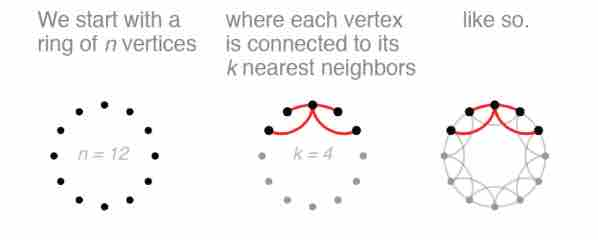
\includegraphics[width=0.5\linewidth]{figures/strogatz.png}
    \caption{Watts-Strogatz model (\href{https://www.kth.se}{source})} % should include the precise source
    \label{fig:watts-strogatz}
\end{figure}

When $n>2k$, there are in total $nk$ edges in the network, which remains constant throughout the rewiring process.

\begin{remark}
    Instead of a ring in with $n$ equal spaced vertices $\real^2$, we can also start with a torus in higher dimensions. For example, in $\real^3$, we fold a square lattices of $n^2$ vertices into a torus.
\end{remark}  

One of the most popular modification of Watts-Strogatz is the \textbf{Newman-Moore-Strogatz} model, where instead of rewiring, we introduce random shortcuts:
\begin{itemize}
    \item Start with a ring of $n$ vertices, where each vertex is connected to its $k$ nearest neighbours.
    \item Add shortcut between $v$ and $u\notin \text{bd}(v)$ with probability $p$.
    \item Repeat for some iterations.
\end{itemize}

This gives an exact degree distribution with $d(v) \sim 2k+\mathrm{Binom}(n-2k-1, p)$.

However, the degree distribution of real world networks often follows a power law, i.e. $p(d)\sim d^{-\gamma}$ for some $\gamma>0$.  

\begin{remark}
    Intuitively, the power-law distribution says that vertices tend to attach to "popular" vertices.
\end{remark}

\subsection{Barab\'{a}si-Albert}  

\begin{definition}
    A probability measure with p.d.f. $p(d)$ is said to follow a \textbf{power law} if there exists $\gamma>0$ and some constant $C>0$ such that $p(d)\sim C d^{-\gamma}$ as $d\to \infty$, where $\gamma$ is called the \textbf{power-law exponent}.
\end{definition}

To explain this power-law behaviour, Albert and Barab\'{a}si proposed the \textbf{preferential attachment model}, which has the following construction:
\begin{itemize}
    \item Start with $m_0$ vertices, the edges between which are formed arbitrarily.  
    \item (Growth) At each time $t$, add a new vertex with $m\leq m_0$ edges that connect to $m$ existing vertices.
    \item (Preferential attachment) The probability that the new vertex connects to vertex $v_i$ is given by:
    \begin{equation*}
        \pi_i = \frac{d(v_i)}{\sum_j d(v_j)}
    \end{equation*}
\end{itemize}

The resulting graph may contain self-loops and multi-edges. A more mathematically rigorous way to define this model is given in \citep{barabasi2016network}.  

\begin{unexaminable}
    To see why the distribution of degrees follows a power law, we consider a continuous-time approximation to the degree of vertex $v_i$, denoted by $k_i(t)$. Then the rate of change is given by:
    \begin{equation*}
        \frac{d k_i}{dt} = m \frac{k_i}{\sum_j k_j}
    \end{equation*}
    But noting that $\sum_j k_j = 2mt - m$, we can solve this equation  to obtain:
    \begin{equation*}
        k_i(t) = m \left( \frac{t}{t_i} \right)^{\frac{1}{2}}
    \end{equation*}

    where $t_i$ is the time when vertex $v_i$ is added (we used the initial condition $k_i(t_i)=m$).

    To compute the degree distribution, note $\Pr(k_i(t)>k) = \Pr(t_i < \frac{m^2}{k^2} t) = \frac{m^2}{k^2}$, if we assume the vertices were added uniformly over time: $t_i \sim \mathrm{Unif}(0,t)$. Now differentiating with respect to $k$, we obtain:
    \begin{equation*}
        \Pr(d(v_i)=k) \approx 2m^2 k^{-3}
    \end{equation*}
    for $k$ large. This is a power law with $\gamma=3$.
\end{unexaminable}



\subsection{Configuration Model}

\subsection{Chung-Lu}

\subsection{Geometric Random Graphs}

\subsection{Expontnial Random Graph Models}




\bibliographystyle{apalike}
\bibliography{bibliography2.bib}




\end{document}